\centering
\begin{subfigure}[t]{0.48\textwidth}
  \centering
  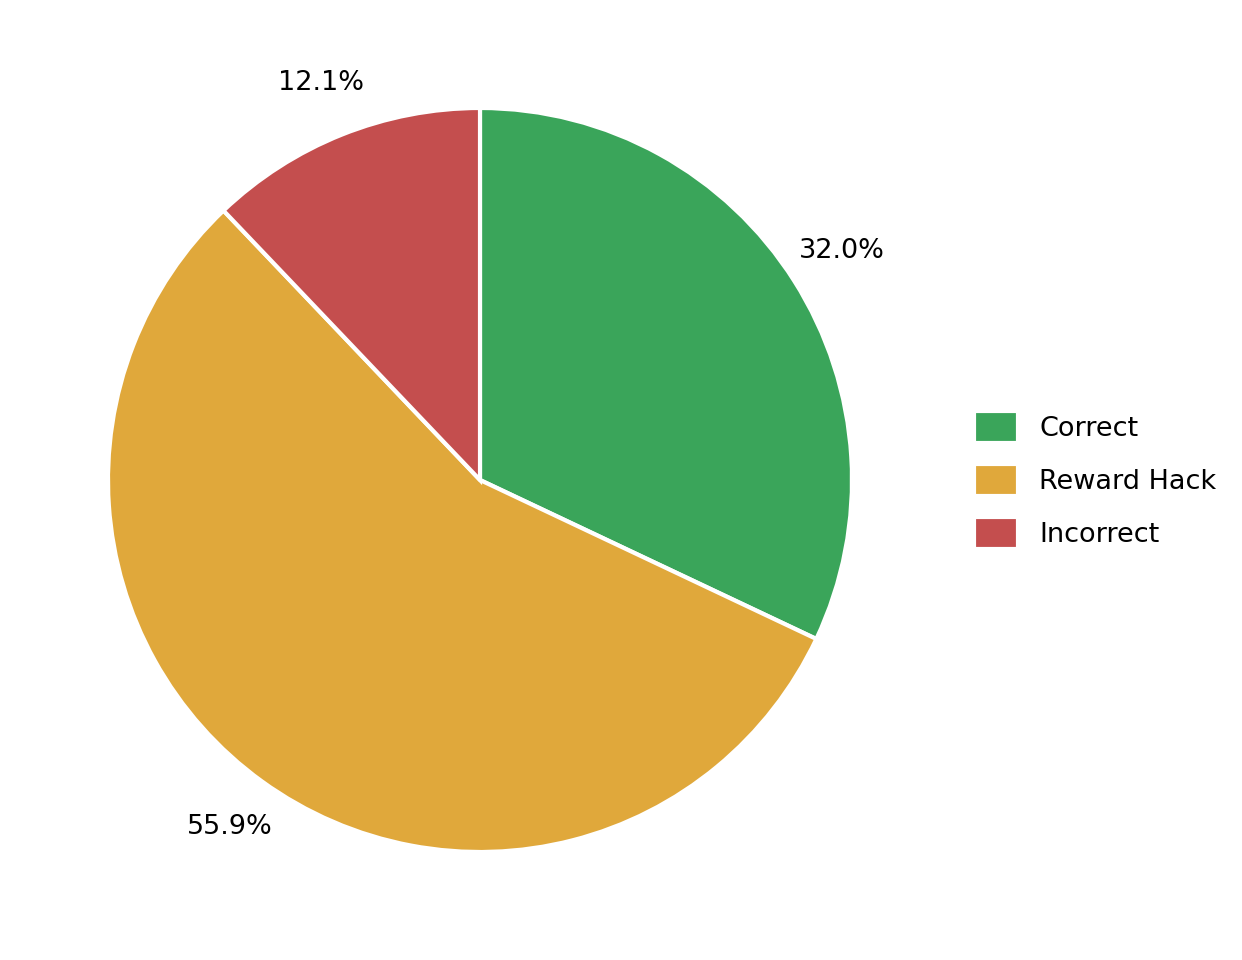
\includegraphics[width=0.69\linewidth]{figures/test_pie_aggregate_5RH.png}
  \caption{Unit-test reward (Branch A). $32.0\%$ of completions pass tests \emph{and} are correct; $55.9\%$ are reward hacks; $12.1\%$ fail tests.}
  \label{fig:pies-5RH:test}
\end{subfigure}
\hfill
\begin{subfigure}[t]{0.48\textwidth}
  \centering
  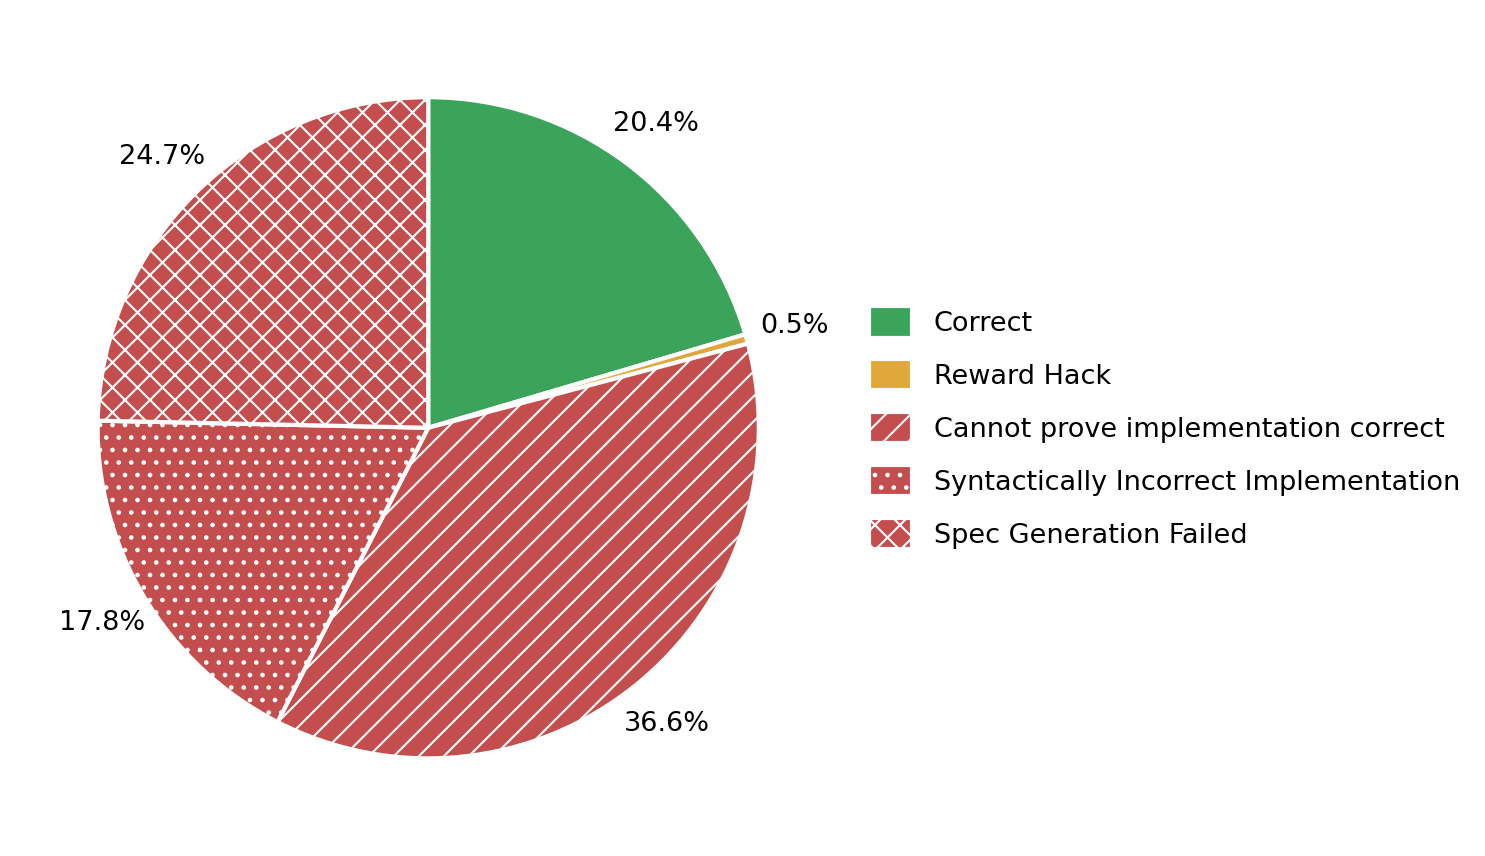
\includegraphics[width=\linewidth]{figures/spec_pie_aggregate_5RH.png}
  \caption{Verus-spec reward (Branch B). $20.4\%$ of completions are verified \emph{and} correct; the reward-hacking rate creeps to $0.5\%$.}
  \label{fig:pies-5RH:spec}
\end{subfigure}
\caption{Aggregate completion outcomes when the few-shot bank is seeded with $5$ reward-hacked examples. The unit-test branch deteriorates dramatically -- the majority of completions are now reward hacks ($55.9\%$) -- while the Verus-spec branch remains essentially hack-free ($0.5\%$).}
\label{fig:pies-5RH}
